\section{Existing Neuropsychological Measures of Cognitive Impairment, and Repeatable Battery of Neuropsychological Tests}
In terms of standardised cognitive tests there are two main aims. Does the test distinguish accurately between normal aging, MCI and AD (diagnostic utility) and does the test distinguish between those individuals with MCI who will then go on to develop AD and those individuals with MCI who don't then go on to develop AD (prognostic utility). This section of the literature review outlines a number of different cognitive tests that have been used to measure cognitive impairments as well as their performance in terms of both diagnostic and prognostic utility.
\par 
\subsection{Repeatable Battery for the Assessment of Neuropsychological Status}
The Repeatable Battery for the Assessment of Neuropsychological Status (RBANS) was originally developed as an assessment tool for dementia, specifically looking at detecting a characterizing very mild dementia \cite{Randolph1998}. The authors felt that there was a shortfall of appropriate measures that were sensitive enough to milder impairments as well as a number of other shortcomings of existing tests. They met a number of design goals for this new battery of tests that addressed these shortcomings. The RBANS consists of a number of sub-tests across five distinct domains.

\begin{enumerate}
	\item Immediate Memory 
	\begin{enumerate}
		\item{List Learning}
		\item{Story Memory}
	\end{enumerate}
	\item Visuospatial / Constructional
	\begin{enumerate}
		\item{Figure Copy}
		\item{Line Orientation}
	\end{enumerate}
	\item Language
	\begin{enumerate}
		\item{Picture Naming}
		\item{Semantic Fluency}
	\end{enumerate}
	\item Attention
	\begin{enumerate}
		\item{Digit Span}
		\item{Digit Coding}
	\end{enumerate}
	\item Delayed Memory
	\begin{enumerate}
		\item{List Recall}
		\item{List Recognitions}
		\item{Story Memory}
		\item{Figure Recall}
	\end{enumerate}
\end{enumerate}

However, whilst the authors claim that the RBANS is adequately sensitive in person's with MCI \cite{Randolph1998} and there is some research to support this assertion \cite{Karantzoulis2013}, other research points out that the RBANS has poor sensitivity in detecting MCI \cite{Duff2010}. Another drawback of this battery is the lack of executive function measures and object naming tasks. Research has shown that the RBANS has good test-retest reliability and convergent validity. However, Duff et al warned that caution should be exercised when using the RBANS in a MCI population as it has lower sensitivity in this population \cite{Duff2010}.

\subsection{Digit Span Test}
The Digit Span Test (DST) is predominantly used to measure a person's working memory capacity, specifically the capacity used to store and recall numbers. A participant is presented with a series of numbers of fixed length and is asked to recall those numbers in normal or reverse order. The series of numbers gets progressively longer until such time as a participant fails three or more times out of eight presentations.
\par
Research has consistently shown that MCI patients have a significantly lower digit span score in both normal and reverse order versions of this test and a study by Muangpaisan has shown that the reverse order version of this test can, to some degree, predict a diagnosis of MCI \cite{Muangpaisan2008}. Muangpaisan also found that Age, Gender and Education have an impact on the performance of the tests. Emrani et al found that the DST revealed no differences between specifically amnestic MCI and controls, but could differentiate between Mixed MCI and the other groups with mixed MCI recalling fewer correct responses than other groups. Notably, there was an attenuated recency effect in those with mixed MCI. \cite{Emrani2018}. Kessels identifies that that there are working memory deficits in MCI patients and these worsen with AD patients. \cite{Kessels2011} He also identified that both MCI and AD have impaired performance on all three conditions of the digit span test. No differences were found between forward and backward conditions in any of the groups. However, available tests may not detect subtle impairments \cite{Kessels2015}.
\subsection{Rey Auditory-Verbal learning test}
Rey's Auditory Verbal Learning Test (RAVLT+) looks a wide range of neuropsychological processes including short-term auditory-verbal memory, learning and retention of information. Participants are given a list of 15 unrelated words, repeated over five different trials and are asked to repeat. Another list of 15 unrelated words are given and the client must again repeat the original list of 15 words and then repeat it again after 30 minutes \cite{Schmidt1996}.
\par
Several studies have shown that an impairment in RAVLT score reflect well the underlying pathology caused by AD. Thus making the RAVLT an effective early marker to detect AD in persons with memory complaints. Moradi investigated to what extent the RAVLT scores are predictable based on MRI data using machine learning approaches, as well as to find out what the most important brain regions are for the estimation of RAVLT scores \cite{Moradi2017}. They found a highly significant cross validated correlation between the estimated and observed RAVLT immediate and RAVLT Percent Forgetting. Further, they found that the conversion of MCI subjects to AD in 3-years could be predicted based on either observed or estimated RAVLT scores with an accuracy comparible to MRI-based biomarkers \cite{Moradi2017}. Another study by Schoenberg found that RAVLT to best distinguish patients suspected of Alzheimer's disease from the psychiatric comparison group \cite{Schoenberg2006}.
\subsection{Digit Symbol Substitution Test}
The Digit Symbol Substitution Test (DSST) involves a key consisting of the numbers 1-9 and a corresponding unique symbol. Below this key is a series of numbers from 1-9 in a randomized order and repeated multiple times. The participant is asked to fill in the corresponding symbol for each number. The task requires that the participant move between the key and the randomized sequence such that  they may retrieve the correct answer from the key, hold this in short-term memory and transcribe the key in the appropriate place.
\par 
Among those with no disorder in cognition, mobility and mood, being in the lowest DSST quartile compared to the highest was associated with nearly twice the odds of developing one or more clinical or subclinical disorders. Associations were stronger for incident clinical disorders in cognition. Slower psychomotor speed may serve as a biomarker of risk of clinical disorders, mobility and mood. While in part attributable to vascular brain disease, other potentially modifiable contributors may be present \cite{Rosano2016}. Further studying the causes of psychomotor slowing with ageing might provide novel insights into age-related brain disorders. Pascoe compared patients with PD with Normal Cognition (PD-N) with those with PD and MCI (PD-MCI) and healthy participants. PD-MCI participants achieved significantly lower scores than other groups in the DSST task \cite{Pascoe2018}.
\subsection{Verbal Fluency}
There are a number of tests that characterise this category of verbal fluency, but generally fall into two categories. Letter (Phonemic) fluency involves the generation of as many words as possible which begin with a specified letter. Category fluency involves the generation of as many words as possible that fall into a specfied category. Both these tasks impose demands on a number of different cognitive processes namely, executive function, verbal retrieval and recall, giving appropriate answers while monitoring previous answers and inhibit inappropriate responses. However, these two tasks require different strategies when attempting them. Letter fluency relies on search strategies based on lexical representations whereas category fluency requires a search for semantic extensions of a superordinate term, meaning that semantic associations within the lexicon must be intact in order for the task to be carried out successfully. 
\par  
There have been numerous studies which have documented the impact that AD has on verbal fluency tests in both categories. A review carried out by Henry et al \cite{Henry2004}, found that performance in both letter fluency and category fluency was impaired in those with AD vs controls, but found a larger effect for tests of semantic fluency.
\subsection{Naming Tests}
Word-finding difficulty is a common symptom of AD and these deficits usually occur during the early stages of the disease progression. As such , a test of a patients ability to find words (known as confrontation naming) is a common way to measure cognitive decline. One common way to do this is the Boston Naming Test (BNT) which comprises 60 items on a spectrum of very frequent to very infrequent. This has been reduced subsequently to two thirty item versions and four fifteen item versions, which correlate significantly with the original sixty item version and the benefit of the shorter versions of the test is that it facilitates testing of individuals with AD who may suffer from fatigue or limited attention span \cite{Williams1989}.
\par 
Willers et al \cite{Willers2008} studied Twenty aMCI patients, twenty AD and 21 controls matched by age, sex and education level. They found AD patients obtained significantly lower total scores on the BNT than aMCI patients and controls. aMCI patients did not obtain significant differences in total scores but showed significantly higher semantic errors compared to controls. Semantic processing is impaired during confrontation naming in aMCI.
\par 
Vadikolias investigated the impact of education on naming tests \cite{Vadikolias2012} and found that higher educational attainment in aMCI subjects were correlated with better performance in verbal and non-verbal tasks during repeated examinations over 1-year. Subjects with a lower level of education performed worse than patients with a high level of education who presented a more stable clinical score. The explanation for this is the idea of a 'cognitive reserve' in participants with a higher education such that this provides a buffer that, while not preventing the physiological symptoms of AD, can potentially delay the clinical onset of cognitive symptoms that characterise AD. This theory is supported by Snowdon who found a relationship between early life linguistic ability and the density of neurofibrillary tangles in his nun study \cite{Snowdon1996}. Whilst these studies and tests provide evidence that there are word finding difficulties in those with MCI, on their own they do not provide sufficient ability to diagnose MCI or provide an prognosis of disease progression.
\subsection{Rey-Osterrieth Complex Figure Task}
The Rey-Osterrieth Complex Figure (ROCF) is a task widely as a test of visuo-spatial skill and visual memory. The task, which was originally designed by Rey (1944) and standardised by Osterrieth (1944) \cite{Rey1941, Osterrieth1944}, asks a participant to copy a complex geometrical figure (known as the immediate copy condition and to recall and reproduce the figure from memory without warning (known as the delayed recall condition). In the immediate copy condition, the complexity of the figure requires an integrative cognitive ability. The reproduction of such a complex structure involves processes such as planning and organizational strategies that are related to executive functions. In order to make this task repeatable, Taylor et al designed a comparable set of figures which have proven to be of equivalent difficulty \cite{Taylor1969, Strauss1990}. 
\par
Salvadori found that patients with vascular MCI had a worse performance in the immediate copy of the ROCF compared to individuals with degenerative MCI, despite their significant impairment in terms of general cognitive status and visual memory \cite{Salvadori2018}. Evidence shows that patients with disorders that possibly involve attention and executive functions are characterized by a more disorganised approach when copying the ROCF compared to controls. One of the difficulties with the presentation of this task in a repeated battery will be the fact that it turns from an incidental memory task (it is a memory task but the participant is not forewarned that they will be required to memorise the picture) into an intentional memory task (given the previous exposure to the task, it would be expected that a participant would preempt the delayed recall portion of the test and spend more time attempting to memorise the details) \cite{Teng2009}. 
\subsection{Hayling Sentence Completion Test}
Inhibitory deficits are a common in all stages of dementia. This is usually tested using Stroop test, however this has the drawback of lacking ecological validity. Therefore researchers have moved towards using the Hayling Sentence Completion Test (HCST) which uses skills such as word retrieval as well as the ability to inhibit ones responses where appropriate and is therefore a much more ecologically valid task. There are two parts to the HCST. In the first part, participants have to complete a sentence by providing a word that best fits the given sentence (this is known as the initiation condition). In this second part, participants have to complete sentences by inhibiting an impulse to give the word that best first the sentence as in the first part, and producing a semantically unconnected word. Performance in both conditions is measured by the time taken for the participant to initiate a response, and in the inhibition condition also by the correctness of the word.   
\par 
Martyr et al compared healthy controls with patients with dementia and patients with Parkinson's disease \cite{Martyr2017}. They found that a high proportion of Category A errors (producing a word that fits the sentence when instructed otherwise) was a factor in performance loss for participants with dementia. Findings suggest that the HSCT may be sensitive to verbal suppression deficits and may provide insight into inhibitory control in participants with dementia. Patients with Dementia were significantly slower than controls in the initiation and inhibition conditions vs healthy controls, and slower than patients with Parkinson's disease in the initiation but not the inhibition condition.
\subsection{Grooved Pegboard Test}
The Grooved Pegboard Test (GPT) was originally designed to cover a variety of different psycho-motor functions including hand-eye coordination and motor speed. However, some studies have shown a correlation of performance in the GPT and measures of cognitive performance such as the Montreal Cognitive Assessment.
\par 
Bezdicek found that the GPT predicted performance on the MoCA and concluded that in addition to being a measure of motor skills, there were results that showed that the GPT could also provide information about a participants cognitive skills \cite{Bezdicek2014}. Whilst this was specifically using a population of patients with Parkinson's disease, given the MoCA and GPT have shown degree of correlation, there remains an opportunity for research that explores the use of the GPT with MCI and Early AD populations.
\par 
Darweesh et al, used the Purdue Pegboard Test (PPT) to assess manual dexterity in a healthy older adult population and followed their participants for between eight and twelve years until an indication of the onset of a neurodegenerative disease \cite{Darweesh2017}. In this time 227 (4\%) of their participants went on to develop a diagnosis of dementia. They noted that higher PPT scores were associated with lower risk of incident neurodegnerative disease and noted significant associations of PPT scores with all forms of dementia and this potentially highlights a deterioration of motor function in the pre-clinical phase of dementia.
\subsection{Visual Search}
The visual search task requires participants to be watching a computerised display in which a target appears either by itself or surrounded by other elements which are used as a distraction. These other elements can be vary in similarity to the target. This is inherently a measure of attention shifting and processing of various similarity and as one would expect, the visual search time is increased in the presence of distractors. This effect is magnified in participants who have a cognitive impairment. 
\par
Research has shown there to be deficits in both AD and MCI populations in this task \cite{Tales2005}, and those with MCI exhibited less severe deficits compabut that these deficits were not as apparent in MCI populations, there remained a significant enough difference that could be used to differentiate healthy controls from those with MCI. In a comparison of visual search performance between those with aMCI and healthy controls, Tales noted significantly poorer performance in the aMCI group. However, she also noted a good deal of heterogeneity in the aMCI group which illustrates that whilst the aMCI group have essentially the same condition, presentations within this population can differ markedly. The results from this study also illustrates the use of a non-memory task as a means of diagnosing dementia as patients who went on to be diagnosed with dementia whilst this study was in progress had significantly poorer visual search performance.  
\subsection{Free Cued Selective Reminding Test}
The Free Cued Selective Reminding Test (FCSRT) was borne out of the premise that by controlling the conditions of learning, a measure of memory is possible that is not confounded by normal age related changes in cognition. Theoretically speaking, any controlled learning test should be able to discriminate between cognitive decline due to age and cognitive decline due to a cognitive impairment. The FCSRT starts with a learning phase in which participants are asked to look at a card containing four pictures (e.g., grapes) for an item that belongs to a named category(e.g., fruit). After these four items are identified, immediate cued recall of these four items is tested and this is repeated for a total of 16 items. Following this learning phase is the recall phase in which participants are asked to recall all the items identified without cues and any items which are not recalled are then cued. There are three outcome measures for this test, free recall (the number of items recalled without cues), total recall (the number of items recalled with or without cues) and cue efficiency which is identified as follows \cite{Grober2010}.
\begin{equation} \label{x1}
CueEfficiency = (totalRecall-freeRecall)/48-freeRecall, range 0.0-1.0)
\end{equation}
Grober found that patients with impaired free recall with four times more likely to develop dementia than those with intact free recall \cite{Grober2010}. This test has also been shown to distinguish patients with MCI who then went on to develop AD, from those with MCI that did not then go on to develop AD and this led the researchers to used the test to categorise prodromal or the amnestic syndrome of the medial temporal lobe by FSCRT score \cite{Sarazin2007}. 
\subsection{Conclusions}
I have looked at a number of different cognitive tests and a battery of tests that aim to have high diagnostic and prognostic capabilities in the MCI population. However, particularly with the RBANS, there lacks sufficient sensitivity in differentiating those with MCI from healthy elderly individuals such that this tool could be used with a level of confidence in a clinical setting. In regard to the tests, a common theme is a lack of studies and therefore evidence into the utility of these tests with an MCI population. However if, as researcher, we aim to investigate this population further then a benchmark battery of tests which is sensitive enough in both diagnostic and/or prognostic utility should be a goal. 
\par 
Another criticism of the current literature is the lack of consistency with regard to the experimental groups. For example, some studies focus on differentiating between an MCI group, a AD group and a healthy controls group whereas other studies may further subdivide the MCI category according to a number of factors such as Amnesic or Non-Amnesic MCI, Mixed MCI (sometimes called Multi-domain MCI in the literature). Given the inconsistency in defining the experimental groups the confusing and often conflicting results that researchers produce is to be expected. Future research should look at the standardization of the operational definition of cognitive impairment in MCI may result in more consistent predictions of progression to AD. 
\par 
Finally, it can be said that in testing for MCI and comparing these results with a cohort of those with a similar diagnosis has limited utility. This is because there is huge variability in the presentation of MCI within participants that even if controlled for with a matched pairs design for age, gender and education will produce inconsistent results. There is an argument therefore for the use of longitudinal studies, where the comparisons on the performance of these tasks are with the participants themselves. There are not many studies which use a longitudinal approach, although those that do show promising results.

\section{Types of Language Assessment}
One of the key debates when looking at how to analyse language is the type of task provided to elicit language production in participants. In the literature researchers have primarily focused on Picture Description tasks but have also suggested other ways in which we might collect data.
\par
\subsection{Picture Description Tasks}
One of the most commonly used tasks to measure language is the Picture Description task. An example of this is part of the Boston Diagnostic Aphasia Examination (BDAE), called the Boston Cookie Theft picture description task \cite{Borod1980}. The Cookie Theft picture (pictured below) depicts a scene of a home typical of the period of time when it was created and would generally not require participants to use any complicated vocabulary to describe. In this task participants are asked to describe the picture presented to them in as much detail as possible.  This task was originally designed to assess Aphasia, but has shown itself to be useful in the assessment of language for the purposes of diagnosis of MCI and AD as well \cite{Giles1996}
\begin{figure}[H]
\centering
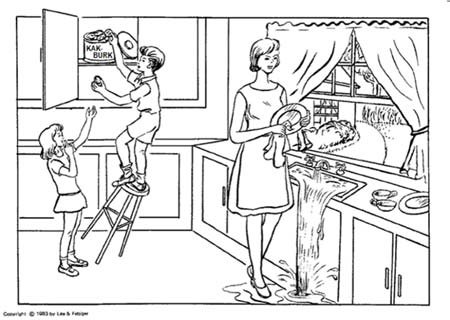
\includegraphics[width=240px, height=150px]{images/BCTPicture.png}
\caption{Cookie Theft Picture - From Kaplan and Goodglass (1983)}
\end{figure}
\par
The picture description task does a fine job of eliciting descriptive language however because of the specific content the language produce could be considered quite limited. There is some disagreement as to the benefits of this using this methodology. This task is reported as being useful to lexico-semantic disorders \cite{Boschi2017, Sajjadi2012} as the language being generated is primarly nouns and deixis (words to identify items and words to put those items into context). However, Ash \cite{Ash2012}felt that there was no difference in using this task vs Story Narration (described below). In explaining the differences, it is worth noting that these researchers were using differing variables and this could explain their different perspectives.
\par
\subsection{Narrative description task}
The story narration task is designed to study a participant's ability to describe and elaborate on a story which is depicted using a series of pictures. The stories depicted are usually based on children's books or famous stories with the Cinderella being the one most typically used \cite{Fraser2014}. This task requires ordering the story in a structured and coherent framework. It also requires comprehension and understanding of the stories characters and the events depicted, as well as an awareness of a character's actions, motivations and internal reactions to given events. This task is particularly useful as the procedure reduces the demands on memory, due to the participant being able to access the picture book during the description and is therefore able rule out memory as a confounding variable for any results observed. As noted above, Ash \cite{Ash2012} felt that this task was interchangable with the Picture Description task. However, other research felt that this was a studier test of lexical and semantic abilities as well as syntactic complexity because this task requires interpretation and elaboration in additional to a simple description \cite{DeLira2011}. 
\par
Given the relative strengths of the Narrative description task vs Picture description task, there are few pieces of research that have used Machine Learning to analyse features from Narrative picture tasks \cite{Fraser2014}. This could be due to the availability of data and the absence of any meaningful sets of transcripts of participants performing this task. However, this could be an interesting direction to take research in the future to see if features generated from this task could be used to predict MCI or AD.  
\par
\subsection{Interviews}
Interviews can also be used to elicit language in a more natural way by asking questions to guide a conversation between speakers. There are three types of interviews: unstructured, structured and semi-structured. Structured interviews tend to produce very limited speech and therefore has never been used in this area \cite{Boschi2017}. Unstructured interviews are open ended and generally do not conform to any particular pattern. They use generic themes such as family or hobbies to guide the conversation. Whilst this is the most ecologically valid form of conversation and therefore language generation, it's unstructured nature means that the protocol cannot be consistent and therefore reproduced. Semi-structured interviews are therefore preferred over other forms of interview as a middle ground. The semi structured nature of these interviews means that there is some replicability but does not constrain the participant in answering questions.
\par
The analysis of interviews can be difficult to analyse as both the content can vary even between participants, although it can be argued that content should not affect the type of language being generated unless it is narrow topic or the participant is constrained in how they answer a given question. It is also difficult to measure as there are no pre-defined task goals in comparison to the other two methods. Nevertheless, this is the most naturalistic setting for looking at language production and can be used to look at the syntactic and semantic parts of language generation \cite{Sajjadi2012}. There have been some attempts to use interviews to assess language production in AD with promising results \cite{Asgari2017, Guinn2015}.
\par
\subsection{Conclusions}
One can view the different types of tasks above as a continuum where picture tasks represent a much more controllable task with a lot of supporting research but which generates a much more constrained set of language that is atypical of normal speech in terms of the cognitive functions used. 

\section{How do we analyse language, issues and debates}
There are a wide variety of approaches that we can take in the analysis of language and there is no real consensus on the best approach to this particular problem. This section looks at the different ways in which researchers have looked at the problem as well as discussing some of the areas of contention. 
\subsection{Single Word Language tasks vs Connected Language tasks}
Part of the reason we need to pay attention to how we ask participants to generate data is understanding how we wish to analyse the data afterwards. As discussed above, the different methodologies to collect data generate different types of language. There are two main approaches which we have looked at to analyse language, using frequencies of words and combinations of words and measures of syntax and semantics. There are other less common methods of analysing language but these are beyond the scope of this review.
\par
Single word tasks such as the Boston Naming Test and other such standardized language tests generally target a participants word production where this is defined as the ability to form and express words in accordance with certain criteria (see above for a full description of verbal fluency as task). There are a number of benefits to using single word tasks. From a research methodology perspective, using a standardized test allows researchers to target a very specific process in language generation and isolate factors that impact performance in language well. However, this approach does not take into account other cognitive processes that are used in lengthier speech tasks. More specifically, single word language tasks do not look at the interaction between language, executive functions and reasoning abilities. They also do not require the logical and efficient organisation of ideas. 
\par
Connected language tasks, such as the picture description task and interviews described above are much more reflective of the processes involved in natural language generation. They are able to be relatively constrained in the language available to be used, for example in the picture description task, or they can be unconstrained in the form of interviews. But regardless of how they are framed, they are potentially much more useful in terms looking at all the processes involved in language generation with the drawback that you will not be able to isolate specific parts of the language generation process. A review by Boschi et al concludes that analysis of connected speech is potentially useful in guiding clinicians to identify language disorders \cite{Boschi2017} and also highlights the role of NLP and Machine learning in assisting in this endeavour. 
\par
\subsection{Semantics vs Pragmatics}
When navigating the English language it is necessary to distinguish between what a sentence says in both semantic and pragmatic terms. Semantic meaning refers to the meaning of the words in a sentence local only to the given sentence. Another way to put this is, semantics considers the meaning of words without taking into account the context in which these words are spoken. Pragmatic meaning refers looks at the same sentence in terms of words and grammar but takes into account the situation or context in which these words are spoken. Emery in her literature review looks at all levels of language tasks except for pragmatics, however this is an area that should not be ignored. Whilst the study of language from a pragmatic perspective is much more complex, it is perhaps one of the most vital areas to study because of the number of different cognitive processes involved.
\par
\subsection{Semantic Content}
Another approach to linguistic analysis in this field is the idea of measuring semantic content and complexity. According to Emery (2000) \cite{Emery2000} in which she states that Semantic and Syntactic skills deteriorate first in people with MCI and AD. If this is true, then psychological measures of semantic and syntactic skills should be able to pick up signs of deterioration and act as markers for possible MCI and AD. An example of a semantic complexity measure is the concept of idea density. Formally, idea density is defined as the average number of propositions per sentence \cite{Keenan1973} and this was used to successfully differentiate between people who would later go on to develop AD \cite{Snowdon1996}. An example of semantic content measures is Type to Token Ratio (described below) which is used to measure the lexical diversity of a given piece of text and/or utterance.  This has also shown to be effective in differentiating between MCI, AD and Controls, with those with language impairments \cite{Bucks2000} and this has carried through in research involving machine learning \cite{Wang2016, Thomas2013}.
\par
\subsubsection{Type token ratio(TTR)}
Type token ratio (TTR) is the ratio obtained by dividing the types (The total number of different words) by the tokens (the total number of words in an utterance).
\begin{equation} \label{x2}
TTR = numberOfUniqueWords / totalNumberOfWords.
\end{equation}
\subsection{Thematic and Content elements in relation to the Picture description task}
A number of studies looked at the accuracy of picture descriptions using counts of thematic and content elements within a picture. Whilst called diffferent names such as 'pictorial themes', 'relevant observations and 'semantic units', they all represented the same idea. The only difference between the studies was the number of thematic elements that 'scored' correctly. Nicholas et al identified eight thematic elements of the Cookie Theft picture and used the number of elements as an outcome measure in different groups. He found that patients with AD expressed significantly fewer content elements than controls.
\par
Hier, Hagenlocker and Shindler assessed content using a similar list of thematic elements \cite{Hier1985}. They divided their participants into early-stage and late-stage AD, as well as including a control group. The late-stage AD group produced significantly fewer relevant observations than the early stage group, and the AD group combined produced fewer relevant observations than controls. This study was replicated by Lukatela et al \cite{Lukatela1998}.
\par
Smith, Chenery and Murdoch applied Hier's methodology for constructing pictorial 'themes' with the Picnic Scene from the Western Aphasia Battery (WAB) with a control and patients with moderate to moderately severe AD \cite{Smith1989}. The authors found no difference in the number of semantic elements produced but did not that the group with moderate to moderately severe AD took more time and more syllables to communicate these elements.
\par
\begin{figure}[H]
\centering
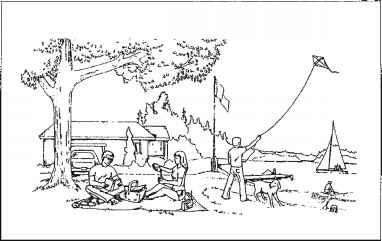
\includegraphics[width=240px, height=150px]{images/picnic-scene.jpg}
\caption{Picnic Scene taken from the Western Aphasia Battery (WAB).}
\end{figure}
Sajjadi et al examined 10 pictorial themes in picture description the Comprehensive Aphasia Test and found that the group with mild AD produced similar themes than controls \cite{Sajjadi2012}. Bschor et al. (2001) examined Cookie Theft picture descriptions at four stages of AD. They found that whilst each AD group differed significantly from the others and also from controls, the measures were not able to distinguish between MCI and normal controls \cite{Bschor2001}.
\par
Finally, a number of studies used composite measures which contained thematic elements and other unspecified information units resulting in a list of 23 possible information units of the Cookie Theft picture. The authors felt that this provided a wider, more liberal range of relevant content and thus subtler differences could be noted. Studies using these features found some differences between AD and controls, and some could differentiate between different stages of AD.
\subsection{General Information Units or Content Information Units}
Some studies used a more general concept of content, using terms such as "general information units" or "content information units" and this could be defined as "the smallest non redundant meaningful fact or inference,"  and was counted whether or not the information conveyed was specific to the context in which the conversation happened. Giles et al for example studied adults with minimal, mild or moderate AD vs controls and found that adults with AD produced fewer overall information units than controls \cite{Giles1996}.
\subsection{Conciseness of information}1`
Conciseness has been defined as the number of words a speaker uses to express ideas. The theory is that people with AD would need more words to convey ideas because of difficulties with word-finding and compensatory  behaviours such as circumlocutions and repetitions. Conciseness has previously been calculated by dividing the number of ideas expressed by the total number of words in a measure commonly referred to as idea density but also known as lexical index, information content and information unit conciseness index. Snowdon examined written discourse from the Nun study and found that low idea density in early life was associated with reduced cognitive performance in later life \cite{Snowdon1996}. Riley et al extended these findings by concluding that early-life idea density was associated with lower brain weight, higher degree of cerebral atrophy and increased neurofibrillary pathology in later life \cite{Riley2005}.
\par
Ahmed, de Jager et al examined idea density with patients who had confirmed AD post mortem \cite{Ahmed2013}. They found that those with AD produced fewer total semantic units than controls but there was no significant difference between the groups with regards to idea density. The study of "empty speech" by Nicholas et al examined conciseness and specifically looked at empty phrases (defined as common utterances which contribute no relevant information), deictic terms (e.g. "this", "that" without referents), indefinite terms (e.g. "thing" or "stuff"), pronouns without proper noun antecedants, and repetitions. In their study they found that AD patients produced more of these than did controls.
\par
\subsection{Efficiency}
% CITE MURRAY!
Efficiency is the rate at which meaningful information is conveyed over time,  and can be calculated by dividing the total number of information units by the duration in seconds of the speech sample. Smith et al, 1989 found that 18 adults AD produced fewer content units over time on average than controls, he attributed these differences to increased circumlocutions and repetitions in the AD group \cite{Smith1989}. Murray used an similar measure in which fillers, irrelevant words, revisions or false stars, vague or non-specific vocabulary and inaccurate output were group together as 'performance deviations" and were divided by the total number of minutes in the sample. This measure was lower for those with AD than those with depression, and also healthy controls. The authors suggested that discourse information measures may help disentangle the similarities in symptoms of early AD versus depression in older adults. Guinn (2012, 2015) \cite{Guinn2012, Guinn2015} found that 'Go-ahead utterances' - instances in dialogue in which a speaker provides responses do not add anything in a conversation beyond a minimal response, were significantly more frequent in those with AD than healthy controls.
\subsection{Total number of words}
Several studies report that adults with moderate AD produce fewer words than controls on picture description, however other studies found no differences in total words among groups of controls and patients with MCI or AD. Murray and Nicholas et al investigated normal controls, patients with AD and older adults with depression and found no group differences in total words \cite{Nicholas1985}. In contrast, Lira et al found that controls produced more total words than patients with AD but found no difference between mild and moderate groups \cite{Lira2014}.
\par
\section{Syntax and Morphology (Language Form)}
Syntax can be defined as the rules that govern how words can be combined to form sentences, whilst Morphology is the system that governs the structure of words and the construction of word forms. Multiple studies of language decline in dementia included at least one measure of syntax or syntactic complexity \cite{Orimaye2017}. Common constructs included words per clause, grammatical form (measures of an appropriate use of syntactic conjections, tenses, conditionals, subordinate clauses and passive constructions), measures of phrase length and proportions of words in sentences. Some researchers have explored the use of formulaic language in those with dementia, the theory being that well practiced phrases are less effortful and therefore place low load on the cognitive abilities of those with AD. The general hypothesis motivating these studies is that either working memory limitations or semantic memory limitations in AD affect one's ability to use complex constructions.
\par
\subsubsection{N-grams}
One of the first features discussed as a potential predictor of MCI or AD is the n-gram. An n-gram is a contiguous sequence of n items from a given sample of text or speech. The items can be phonemes, syllables, letters, words or base pairs according to the application. For example, given the sequence of words "to be or not to be", this extract is said to contain six 1-gram sequences (to, be, or, not, to, be), five 2-gram sequences (to be, be or, or not, not to, to be), four 3-gram sequences(to be or, be or not, or not to, not to be) and so on. This is useful as, given a large portion of text or speech, we can predict the probability of a word being close by to a given word. A number of researchers have used n-grams as features. 
\par
Asgari, Kaye and Dodge (2017) \cite{Asgari2017} used another form of word frequency measurement. Using recordings of unstructured conversations (with standardized preselected topics across subjects) between interviewers and interviewees they grouped spoken words using Linguistic Inquiry and Word Count (LIWC) which is a technique used to categorize words into features such as negative and positive words \cite{Pennebaker2015}. They were able to successfully used machine learning algorithms to distinguish between these two groups with an accuracy of 84\%. 
\par
\subsection{Formulaic Language}
Fraser, Meltzer and Rudzicz (2015) \cite{Fraser2015} looked at connected speech using the DementiaBank corpus. They found that there were four factors which they identified as important in the classification of participants as either healthy or AD. These four factors were semantic impairment, acoustic abnormality, syntactic impairment and information impairment and were based on existing measures of semantic and syntactic complexity. Zimmerer (2016) \cite{Zimmerer2016} looked at whether language was more formulaic in those suffering from AD. He proposed that those who suffer from AD rely on formulatic sentences, for example 'Noun-Verb-Noun', and this is done to reduce language complexity. He noticed a significant difference in the use of formulaic sentences between AD and Healthy Controls.
\par
\section{Pragmatic Language}
The pragmatic language domain refers to the social rules for language for the purposes of communication including, using language to achieve goals, using information from the context to achieve these goals and using the interaction between people to initiate, maintain and terminate conversations.
\subsection{Coherence}
Coherence, in lay terms, can be defined as the ability to maintain awareness of the topic at hand. It can be separated into local coherence which is related to themes of the immediately preceding utterance and global coherence which looks at how closely an utterance is related to the topic currently being discussed. Chapman et al used picture descriptions of Norman Rockwell prints within a frame analysis, with frames being defined as the context in which the picture is viewed \cite{Chapman1998}. The authors identified aspects of content, including whether the frames of interpretation being offered were typical, atypical, incorrect or had no frame. They also looked propositions supporting frames and propositions disrupting frames as measures of coherence. They examined these variables with early stage AD, old-elderly and normal controls. Healthy older adults and normal controls produced significantly more typical frames and more frame supporting information than the AD group. The authors attributed AD patients' difficulties to memory deficits, attentional deficits, visual perceptual problems, disruption of internalized frame representation, or failure to access frame knowledge.
\par
\subsection{Perseveration}
Perseveration can be broadly defined as the repetition of a response regardless of the absence or cessation of stimulus which could have generated an appropriate response in the first place. A typical example could be the idea of conversation moving from introductions to a more general conversation, someone who has difficulties with perseveration will struggle with the move between social contexts and repeat language that would be more used in an introduction context.
\par 
One study examined verbal preservation in the description of Norman Rockwell prints \cite{Bayles198}. The presented participants with a number of similar pictures that had significantly different contexts and asked participants to describe these prints.  They divided the total number of words within perseverations by total number of words in the speech sample. The authors also calculated rate of perseveration on two other language tasks: confrontation naming and generative naming. In all tasks, the AD group produced significantly more perseverations than controls but there were no significant differences between the two groups in the picture task in isolation. The authors felt that this was because picture description was an easier task, as it was a visual task in contrast to the other tasks which tapped into other cognitive processes.
\par
\subsection{Empty Speech}
Verbal fluency is a term used in neuropsychological contexts generally referring to timed, word-generation tasks, while in speech-language pathology contexts, "fluency disorders" are defined as interruptions in the flow of speaking characterized by atypical rate, rhythm and repetitions in sounds, syllables, words and phrases. "Fluency", in the literature of discourse of adults with AD, typically refers to the smoothness or flow of spoken language. Abnormalities of fluency in this population are typically characterised by filled and unfilled pauses, word repetitions, circumlocutions, and revisions.
\par
The study of "empty speech" by Nicholas et al was one of the first to examine aspects of fluency in the connected speech of persons with AD \cite{Nicholas1985}. They found that adults with AD had significantly more repetitions than controls. Similarly, Bayles and Tomoeda found more aborted phrases, revisions and ideational repetitions in the AD group than in controls \cite{Bayles1983}. Several other studies support the idea that in AD population there are a greater number of repetitions and revisions than in healthy controls. However, there are some studies which contradict these findings\cite{Ahmed2013}.
\subsection{Conclusions}
This section has looked at a number of different attributes which researchers have cited as being important in the detection of MCI and AD. Whilst in some cases there is a broad consensus about a given feature in the vast majority of cases there is some uncertainty. Some of the difficulty lies in different approaches used particularly around the criteria for experimental groups which means that it is difficult to be able to compare studies, like for like, as the populations of the participants being studied vary in subtle or obvious ways. It is important for any studies moving forward to use comparable standards when it comes to their experimental groups, such that the picture can be made clearer.

\section{State of literature into Machine Learning and Natural Language processing techniques}
Diagnosing dementia through language analysis has a large background in terms of psychological research. Increasingly current research has called for the use of machine learning as a way of assisting in the process of diagnosis \cite{Orimaye2017, Boschi2017}. This section will look at what areas of natural language processing (NLP) and machine learning (ML) could potentially be used as tools to help in this domain as well as any research that has applied machine learning to this problem.
\subsection{Natural Language Processing}
Natural Language Processing as a topic can be defined as the intersection between Machine Learning and Linguistics and looks at a number of language tasks, particularly important in this domain is how to enable a computer to process and analyse large amounts of language data. Some other tasks include speech recognition, natural language understanding and natural language generation. Generally speaking, Natural Language Processing (NLP) systems mimic the semiotic perspective on language. That is to say that we can subdivide NLP processes into different components (see Figure 2.3).
\begin{enumerate}
	\item Morphological/Lexical: providing the basic language elements or vocabulary, such as words, their roots and inflections.
	\item Syntactic: for grouping and sequencing elements within samples of language (usually sentences).
	\item Semantic: for knowing the meaning of an utterance, usually defined in terms of the 'truth value' of the logical propositions that are thought to be expressed by sentences.
	\item Pragmatic: for understanding the context and purpose of an utterance.
\end{enumerate}
\begin{figure}[H]
\centering
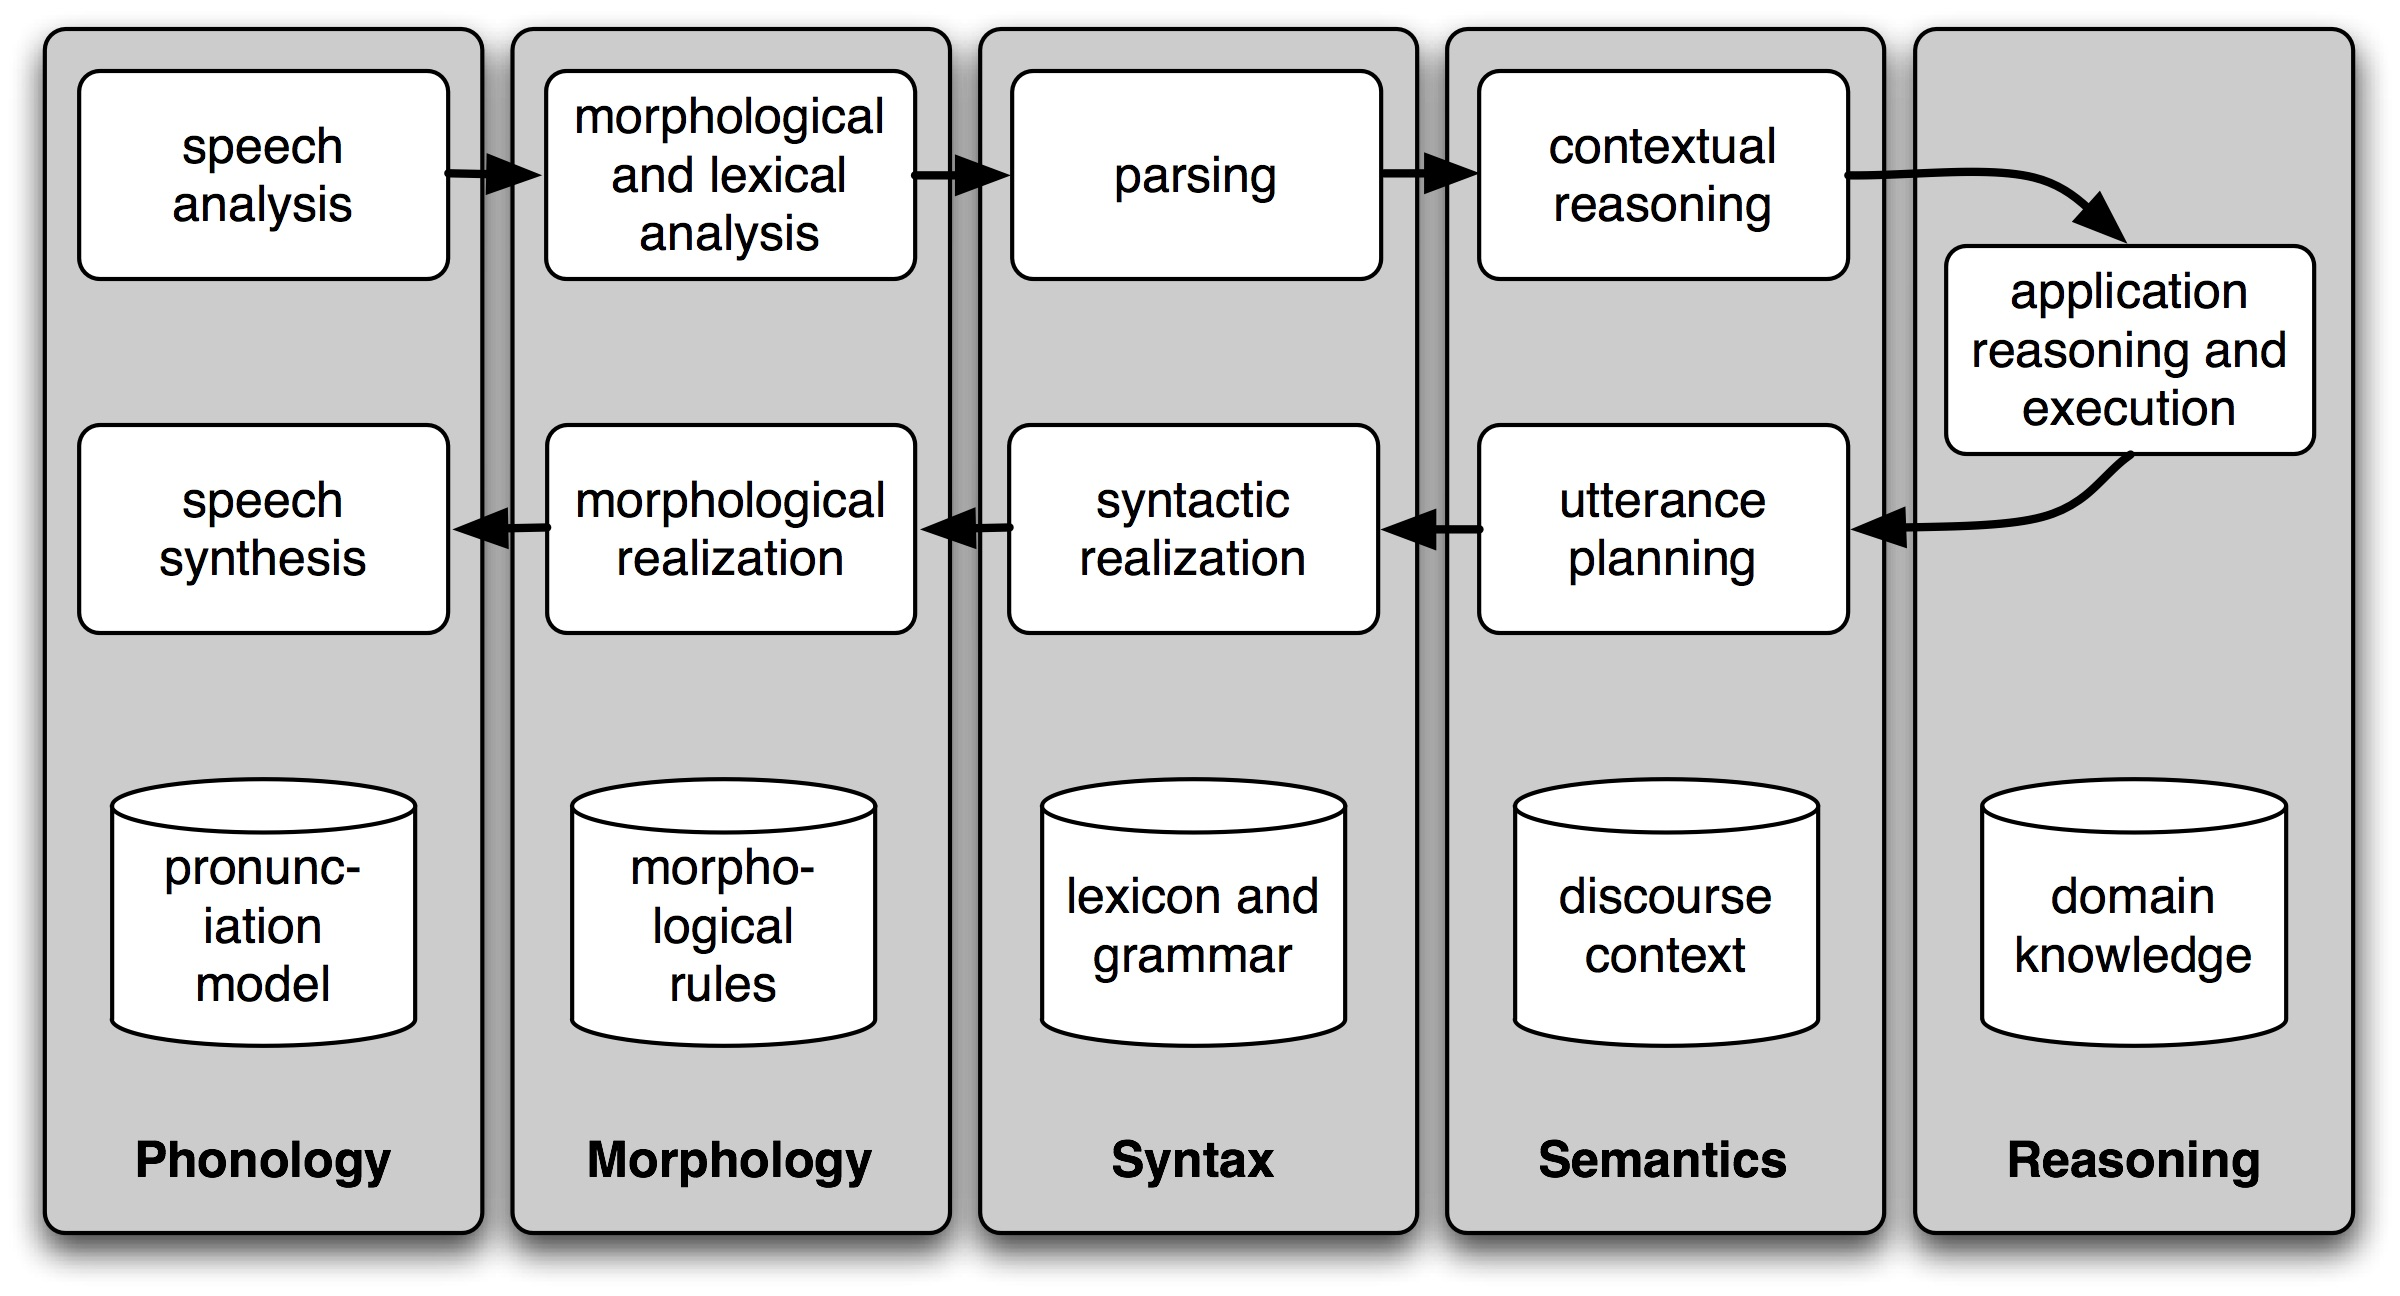
\includegraphics[width=240px, height=150px]{images/workflow.jpg}
\caption{How Natural Language Processing tasks are subdivided.\label{white}}
\end{figure}
In order to facilitate these and other tasks, a number of frameworks have been developed that automate some of the more common processing tasks. A brief review of these frameworks follows. 
\subsubsection{Natural Language Toolkit}
The Natural Language Toolkit (NLTK) was originally designed as part of a computational linguistics course at the University of Pennsylvania but has evolved to become an open-source framework which includes methods and modules for a wide array of Natural Language tasks (see Table 2.2 for a full list) \cite{Bird2009}. 
\begin{table}
	\begin{tabular}{ | p{4cm} | p{7cm} | p{1cm} |}
		\hline
		\textbf{Language processing task} & \textbf{Functionality} \\ \hline
		Accessing corpora & standardized interfaces to corpora and lexicons \\ \hline
		String processing & tokenizers, sentence tokenizers, stemmers \\ \hline
		Collocation discovery & t-test, chi-squared, point-wise mutual information \\ \hline
		Part-of-Speech tagging & n-gram, backoff, Brill, HMM, TnT \\ \hline
		Machine Learning & decision tree, maximum entropy, naive Bayes, EM, k-means \\ \hline
		Chunking & regular expression, n-gram, named-entity \\ \hline
		Parsing & chart, feature-based, unification, probabilistic, dependency \\ \hline
		Semantic interpretation & lambda calculus, first-order logic, model checking \\ \hline
		Evaluation metrics & precision, recall, agreement coefficients \\ \hline
		Probability and estimation & frequency distributions, smoothed probability distributions \\ \hline
		Applications & Graphical concordance, parsers, WordNet browser, chatbots \\ \hline
		Linguistic Framework & manipulate data in SIL Toolbox format \\ \hline
	\end{tabular}
		\caption{\label{tab:table-name}NLTK tasks and functionality}
\end{table}
The NLTK has been successfully used in both teaching and research purposes and as part of this provides access to large array of databases and corpora which have potential uses in common tasks.

\subsubsection{CoreNLP}
Stanford CoreNLP provides a set of human language technology tools. This comes as an installable package that requires JAVA and can be interacted with through the command line or by an accompanying API. Whilst NLTK is much more oriented to parsing text and generating features, CoreNLP does this and adds more functionality such as a Named Entity Recogniser and sentiment analysis functions. At it's centre is the Stanford parser, which parses text and can give the base forms of words, their parts of speech, whether they are names of companies, people, etc., normalize dates, times, and numeric quantities, mark up the structure of sentences in terms of phrases and syntactic dependencies, indicate which noun phrases refer to the same entities, indicate sentiment, extract particular or open-class relations between entity mentions, get the quotes people said, etc.
\par
\begin{figure}[H]
\centering
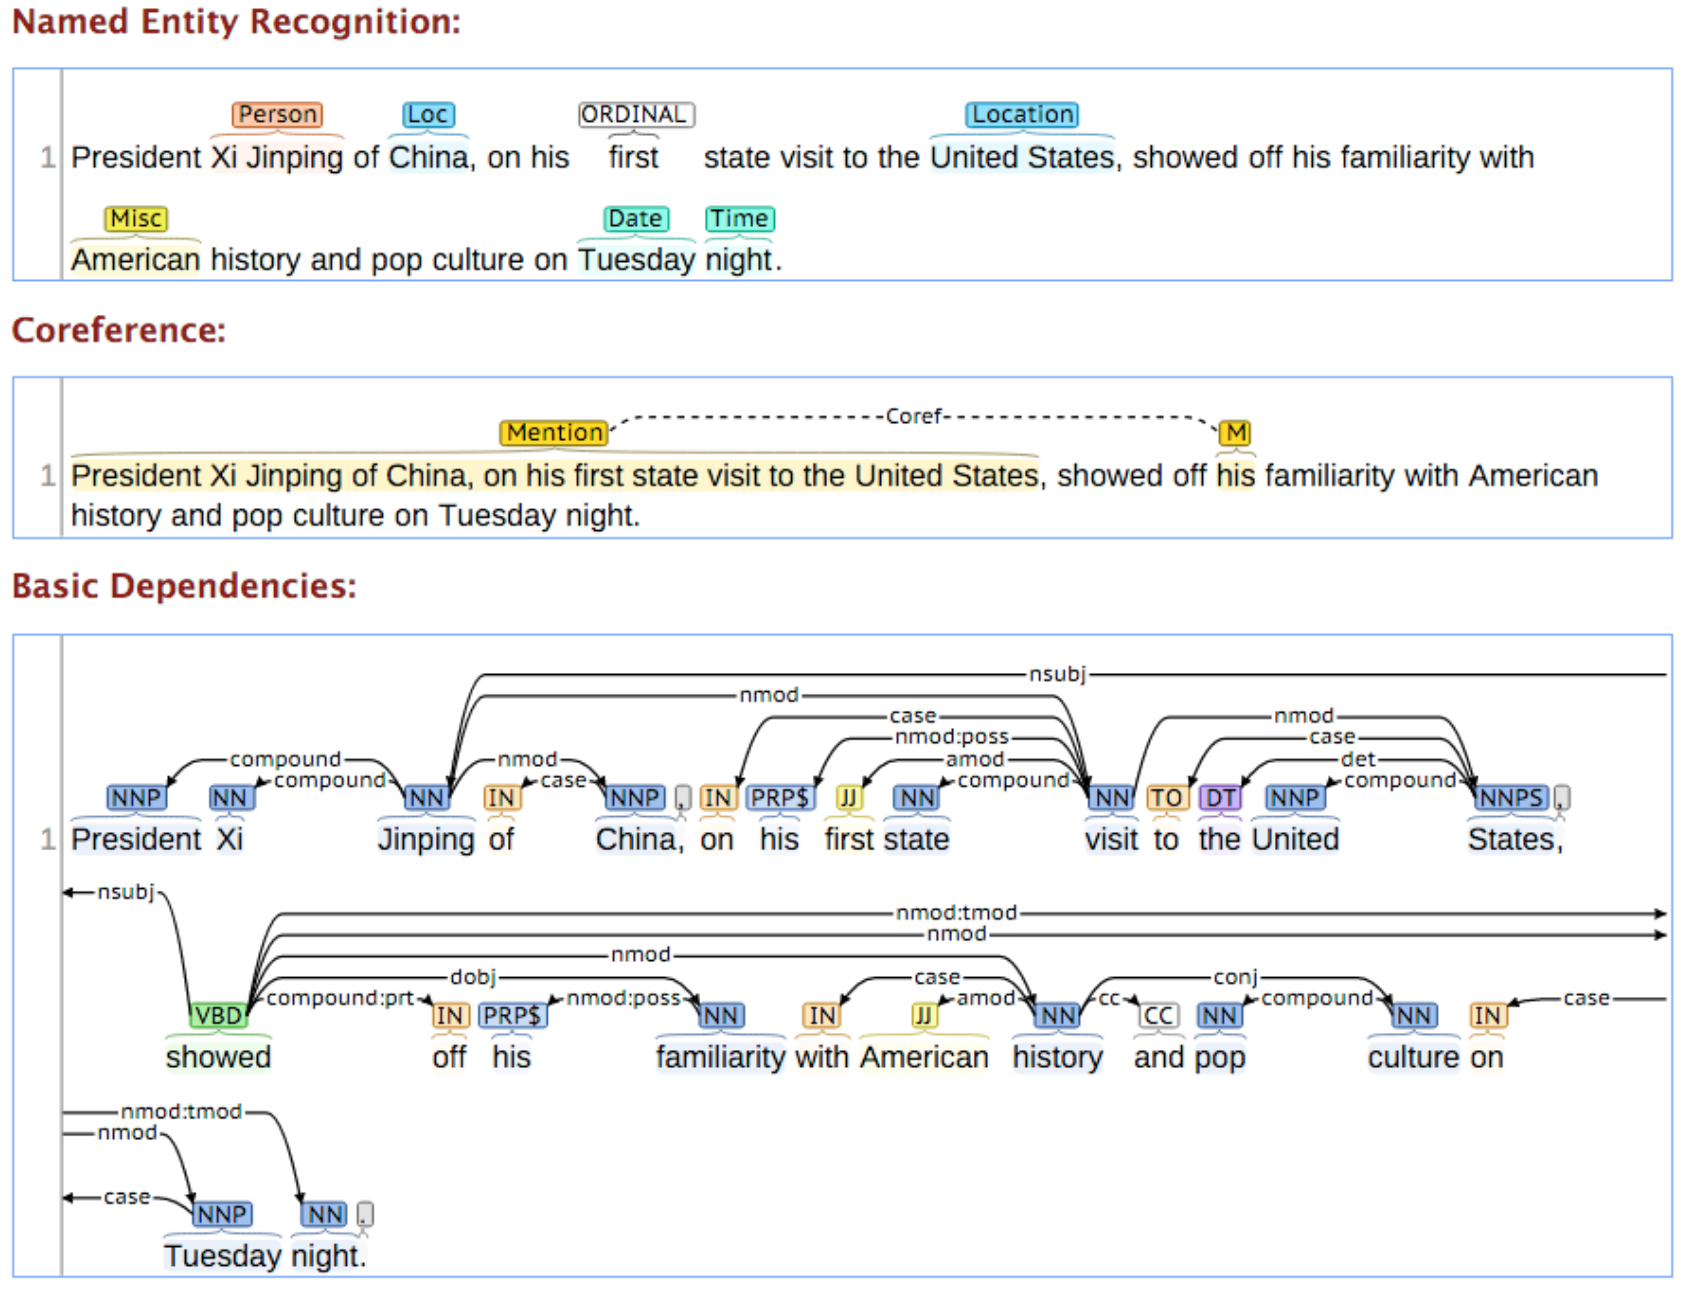
\includegraphics[width=350px, height=200px]{images/CoreNLP.png}
\caption{Depiction of how Core NLP marks up a sentence}
\end{figure}
It's intended for CoreNLP to provide tools and frameworks that will enable higher level language analysis whilst remaining domain agnostic.

\subsubsection{Linguistic Inquiry and Word Count}
The Linguistic Inquiry and Word Count (LIWC) is a piece of software that counts words and assigns these counts to categories \cite{Pennebaker2015}. The rationale behind this is that the words we speak inform an observer of the state of mind of an individual. A typical example of this might be someone with depression who may typically be more inwardly focused and therefore talking in the first person is common\cite{Al-Mosaiwi2018}. The 2015 version of the LIWC has over 90 different categories \cite{Pennebaker2015} and some supporting research suggests that it is effective at identifying themes and associating these themes with mental health difficulties such as depression and anxiety \cite{Sonnenschein2018}. 
\par
Whilst not necessarily a tool that can parse data and look at trends from a linguistic perspective, a framework like this could be used as another tool to explore themes within a persons speech from a more qualitative angle. To the authors knowledge, there is no research that looks at speech changes from this perspective. 

\subsection{Traditional methods of Machine Learning}
In terms of Machine Learning research in this area, a number of researchers have used transcripts based on picture description tasks \cite{Zimmerer2016, Orimaye2017, Mueller2018a, Fraser2015} and have successfully extracted linguistic features that could differentiate between AD and controls.
\par
One of the first attempts to use machine learning and natural language techniques to look was conducted by Thomas \cite{Thomas2005} who was able to successfully demonstrate the ability of machine learning algorithms to analyse n-grams as well as other features to outperform a naive rule-based classifier which always selects the most frequent class. They detail several lexical approaches to the problem of detecting and rating AD. The approaches they looked at relied primarily on character n-gram techniques but also explore correlation of usage of frequency of different types of speech. Their results act as a proof in concept of the utility of using a pure computational approach to the diagnosis of dementia using spontaneous speech. The were able to obtain 95\% accuracy dementia vs controls, 70\% accuracy classifying dementia into two categories and 50\% accuracy classifying dementia into four categories. They suggest further exploration of characteristics to classify \cite{Thomas2005}.
\par 
% Cite CRUM Population-based norms for the Mini-Mental Status Examination by age and educational level
Bucks et al \cite{Bucks2000} took a more traditional approach using frequency rates per 100 words of various word types such as nouns, verbs, adjectives and pronouns and some measures of lexical richness to attempt to discriminate between healthy older participants and participants with probable AD. They found that AD patients had higher mean pronoun rate, adjective rate and verb rate but lower noun rate vs normal older controls \cite{Bucks2000}. It's important to note that the clinical group averaged a score on the MMSE of 15 (sd=6.8) which puts the clinical group in the 'moderately impaired range'. At this stage, the two groups should be reasonably easy to differentiate in terms of language and other cognitive abilities.
\par 
Fraser et al \cite{Fraser2015} built upon the work by Bucks by adding an acoustic analysis element to her analysis using the DementiaBank corpus, as well as significantly expanding the list of linguistic features they used. They used features generated from the Stanford parser (Now known as Core NLP) and computed the frequency of the occurrence of different parts of speech which they then normalised by the total number of words in each utterance. They also computed ratios between these parts of speech such as pronouns to nouns. They also included measures of syntactic complexity such as mean length of sentences and measures of lexical richness such as TTR. Their analysis showed was able to achieve 81\% accuracy in distinguishing individuals with AD from controls based on short samples of speech. They found that there are four factors which they felt were important in discriminating between these two groups: semantic impairment, acoustic abnormality, syntactic impairment and information impairment. 
\par 
Zimmerer et al \cite{Zimmerer2016} took a slightly different approach in that they developed the Frequency in Language Analysis Tool (FLAT) which looked at the degree of formulaicity in an individual sample. The rationale behind this is that people with impaired cognitive function are able to depend on formulaic sentences for language generation to ease the burden of language generation on cognitive symptoms. They were able find that those with probable AD produced more formulaic language than controls. 
\par 
Orimaye et al (2017) \cite{Orimaye2017} investigated the use of machine learning algorithms to detect differences primarily in n-gram use to distinguish between those with a diagnosis of AD and healthy controls. Their main finding supported n-grams as the most significant predictor. One of the criticisms is the use of picture description tasks and n-grams. Because the language generated by this task is content specific the n-grams generated are only specific to the task given and cannot be generalised.
\par 

\subsection{The case for Deep Learning}
One of the criticisms of traditional learning models is it's reliance on features that are generated for them. As we can see from the brief look at some of the research in this field, researchers have taken a number of different approaches with success. However, there does not seem to be a consensus. As machine learning in general moves away from traditional machine learning models to deep learning techniques, it poses the question can deep learning assist with this problem?
\par 
One of the main benefits of deep learning is that it does not rely on pre defined features being fed to the model. Instead, deep learning models take raw data in with some amount of preprocessing and generates it's own features. This move away from relying on features solves one of the difficulties we have with the current psychological literature, namely that there are some disagreement on the which 
\par 
One of the drawbacks of attempting to use natural language processing and machine learning in this context is the lack of data. This is the case with all machine learning techniques, but more so with deep learning. There have been ways to 'create' more data such as data augmentation. 

\subsection{Conclusions}
We can see that both Natural Language Processing and Machine Learning techniques have a lot to offer, Indeed there has been a lot of research which have used pre-existing datasets to explore this area with promising results. One of the difficulties with the current research is the approach of trying to discriminate between those AD and healthy controls. This is not necessarily a problem in the real world as it is trivially easy to do for trained clinicians. A more interesting, but potentially harder to problem to solve is to discriminate between those with MCI and healthy controls, and more importantly to track their decline over time. Further, to date the authors are unaware of any research in which these techniques are applied to newly created samples of language. 

\section{Discussion}
Current state-of-the-art diagnostic measures of AD are invasive (CSF analysis), expensive (neuroimaging), and time-consuming (neuropsychological assessment). Furthermore, these measures are limited to speciality clinics and thus have limited accessibility as frontline screening and diagnostic tools for AD. More importantly, nonspecialists are often inaccurate at identifying early AD and MCI. Thus, there is an increasing need for additional noninvasive and/or cost-effective tools, allowing effective frontline identification of subjects in the preclinical or early clinical stages of AD who could be suitable for monitoring in speciality clinics and for early treatment. Implementation of effective screening instruments will allow diagnosis earlier in the course of dementia, even at the point when memory function is still essentially within the normal range. This strategy would enable an earlier, and potentially more effective, prevention and treatment of AD with a special focus to preserve cognitive functions.
\par 
However the literature has identified a number of challenges when approaching this problem. Firstly, the clinical features that combine to meet the diagnostic criteria for Dementia or it's variants are continuous in nature and heterogenous between patients and are also impacted by other variables. For example as shown above, cognitive performance is affected in part by a patients educational attainment and a patients ability to live independently is impacted by a their physical health as much as their cognitive health. The challenge therefore is to find features that are minimally impacted by other factors, or that can be controlled for by a experimental design such as a matched pairs design to control for educational attainment.
\par 
Another challenge lies with the recruitment of suitable individuals who may notice a decline in cognition to the point where we might classify them as having MCI, but these individuals deduce that there is little to no value to admitting there is a problem and seeking help whilst their symptoms are 'manageable'.
\par
Finally there is a large amount of variability in the presentations of those with MCI and early dementia, and this is compounded by an similar amount of variability in the criteria researchers have used for experimental groups and the approaches researchers have used to tackle this problem. This had led to a confused literature. Recently a call for research that has consistent inclusion / exclusion criteria has been made along with some proposed definitions of MCI and it's subgroups \cite{Petersen2014}. Researchers have identified the analysis of language impairment as an area of promise to explore in the diagnosis of MCI and early AD and recent developments in natural language processing and machine learning techniques have the potential to assist in this research. Indeed, given the increased burden on the diagnosis of MCI and AD on professionals there has been a call to use technology to potentially ease this burden \cite{Boschi2017}. A small but growing amount of research has gone into the use of machine learning techniques to potentially look at the automated classification of participants with MCI and/or AD, however this is a new area of research and there are some gaps in our knowledge.

\subsection{Future Work}
One of the areas for research to study is a careful examination of the features that are being used to measure language deterioration. For example, Zimmerer (2016) \cite{Zimmerer2016} describes connectivity in such as a way that correlates directly with what Mueller (2018) \cite{Mueller2018a} calls Fluency. Whilst these are very nuanced measures which differ slightly in the form they take, the sheer range of measures and features being produced make it difficult to organise and explore what is truly going on in those with MCI and early AD.. Some work needs to be done in producing a consistent list of measures that are validated using existing datasets and can be used for future research moving forward. \newline
\par
Teng et al suggests that work should focus on the MCI population and concentrate on developing a consensus neuropsychological battery that could yield predictable rates of progression to AD \cite{Teng2009}. This, in conjunction with the development of a model of language, sensitive enough to detect subtle deterioration in language use to act as an additional cognitive marker to aid diagnosis could potentially move some way to providing this.
\par 
Future research should also be directed towards developing non-intrusive ways of detecting subtle changes in natural language such that any perceived deterioration that could indicate the presence of MCI or AD could be flagged up early. Machine learning approaches seem to be the most logical approach for achieving this aim as language could be collected in non-intrusive ways and passed to a machine learning algorithm for preliminary classification.  Despite the excellent quality of datasets, for example the DementiaBank dataset, being used to 'backtest' these algorithms, further research should look at generating additional datasets to increase the validity of the results found so far as well as using other methods to generate data other than Picture Description tasks which some researchers could claim are limited in scope. Finally, the recent resurgence in the use of neural networks and deep learning could provide the answer to the confused literature in terms of features. A key benefit of deep learning is it's ability to automate the process of feature engineering. So there is an opportunity to explore the use of deep learning, to not only develop new features but also validate existing features independently.  
\par
This area of research is extremely promising in its early results and the impact of successful research would be life changing for both individuals and the health of the worlds aging population in general.